\section{Description of the algorithms}
\label{sec:Description}

In this section we present the description of the algorithms we have used to eventually find the algorithm that gives the best curve for the set of given points.
We first give some general procedures, then pseudocode for the closed curve, followed by pseudocode for the open curve. Finally pseudocode for the up-to-5 curve is given.

\subsection{General algorithms and datastructures}
\label{sub:general}

Algorithms in this subsection are used by all four subtasks of the curve reconstruction.\\
In each of the algorithms of the subtasks these procedures are called in the process of reconstruction.

\subsubsection{Finding lexicographical smallest point}
As given in the document specifying this problem, the point from which to start the reconstruction is the lexicographical smallest point of the given set of points. To find this point we implemented a data structure to find the minimum of all $x$-coordinates of the points. When there are two points with the same minimum x-coordinate, we look at the $y$-coordinates of these points; the one with the smaller coordinate becomes the lexicographical smallest point of the set (it is not possible they have the same $y$-coordinate, because all points are unique). The running-time of this data structure is $O(n)$ time, because after one walkthrough the array you have found the lexicographical smallest point.

\subsubsection{Storing points and NearestNeighbor algorithm}
We first tried to solve the reconstruction of the curve with only a NearestNeighbor algorithm, in order to do this we needed an algorithm to store the given set of points efficiently. Therefore, we attempted to implement a kD-Tree, because in such a tree you can quickly find the nearest neighbor of a point by traveling down the tree to its leafs. While implementing the kD-Tree, we found out that this was to complex, because there were so many cases you have to take into account. We also got to know that only a NearestNeighbor algorithm does not do the trick, as shown in Figure 1, so we needed more than this.
\begin{center}
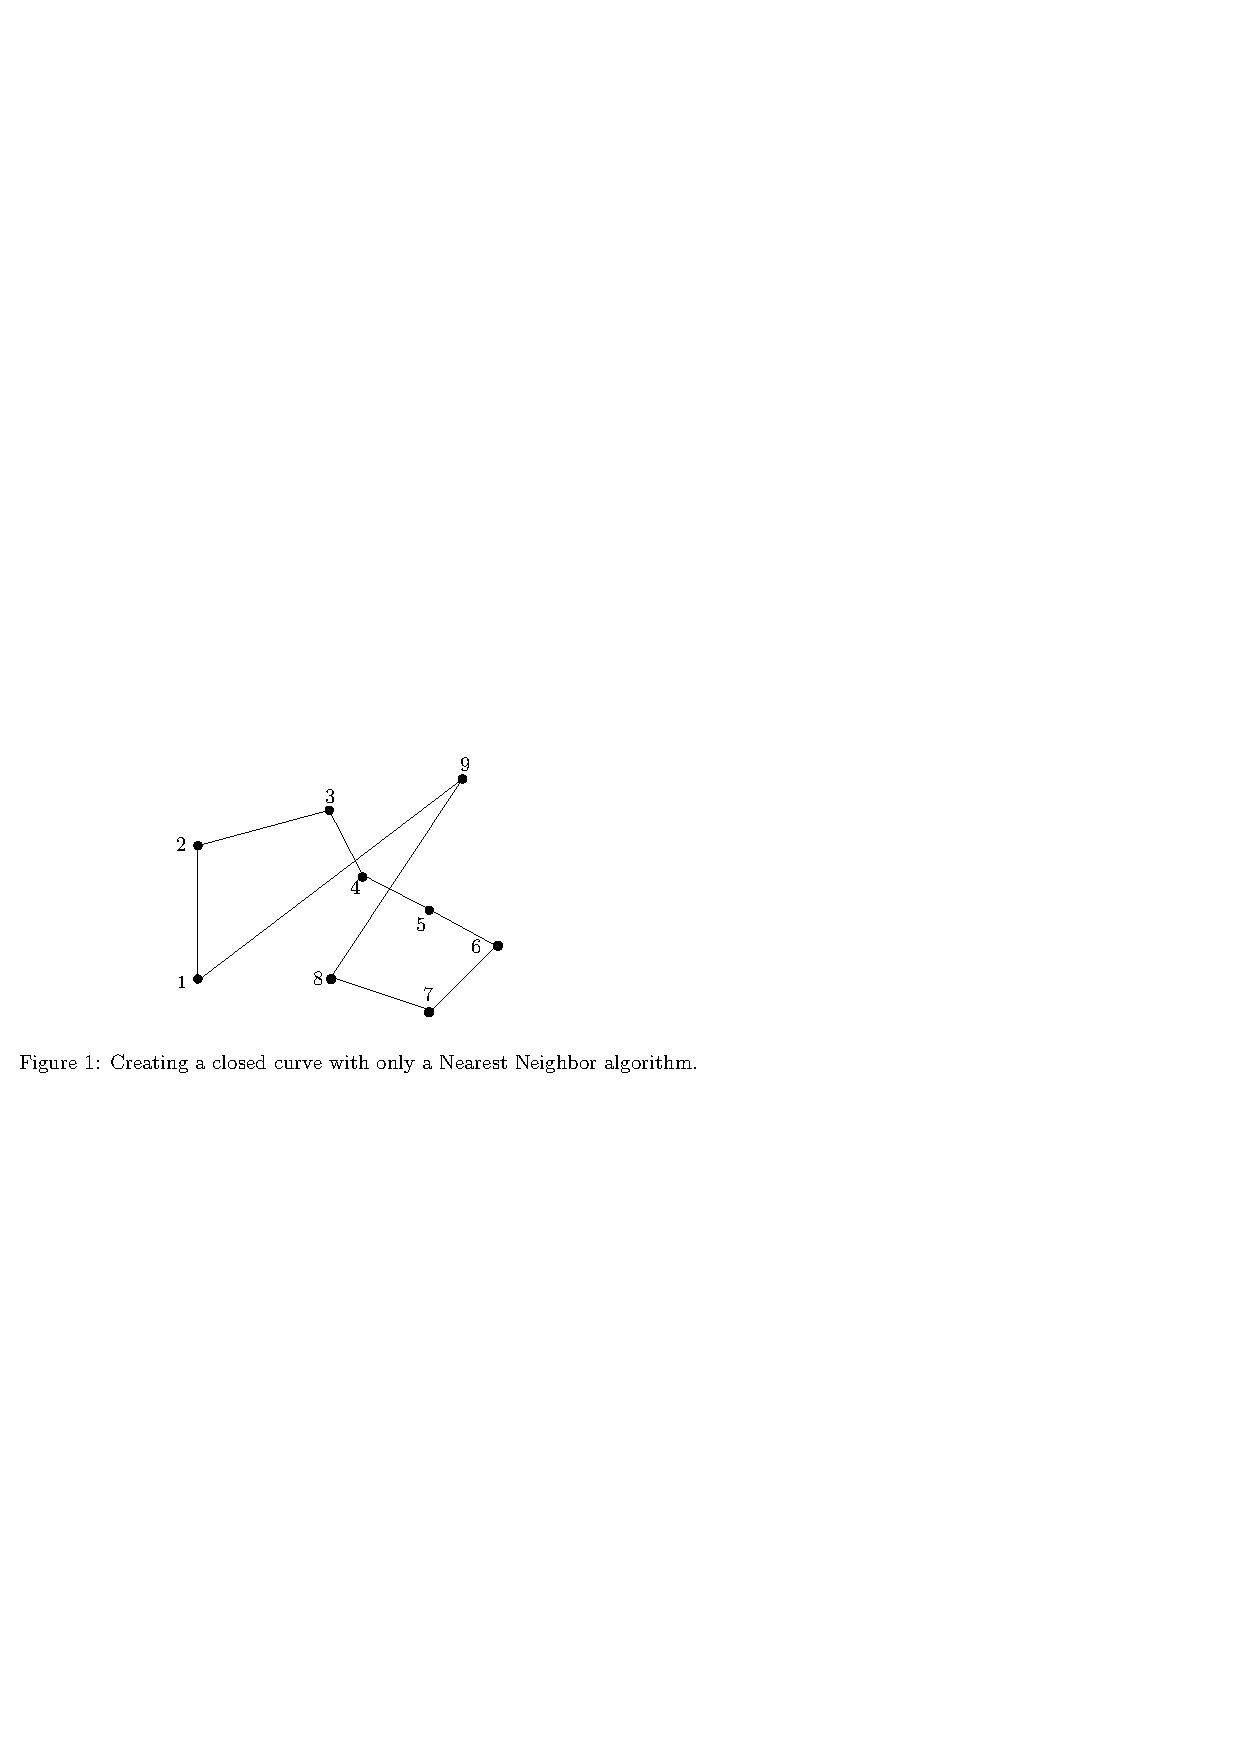
\includegraphics{Description/Figure1}
\end{center}
To keep things simple we implemented an algorithm of our own to search for the nearest neighbor. This algorithm gets a point from the given set as input an goes through all the remaining points to find the nearest neighbor of the input-point.\\
The running-time of this algorithm is $O(n^2)$

\subsubsection{Checking on intersections}
After a curve is (partially) constructed we check on whether or not it contains intersections. In the Open-, Closed- and Up-to-5-curves problems intersections are not allowed, whereas in the Intersection-curve problem at least one intersection has to occur.\\
To find intersections we go through all points after a possible solution is computed. We take all the edges and check whether they intersect or not. Depending on which problem you are addressing, a solution is rejected or accepted.\\
The algorithm computing whether two edges intersect or not takes constant $(O(n))$ time, because its a sequence of assignments to certain variables.\\
To further clarify this data structure pseudocode is given in Figure 2.\\
It gets four points as input.\\

\begin{center}
\includegraphics[scale=0.5]{Description/Figure2}
\end{center}

\subsubsection{Backtracking}
In addition to the previous algorithms we used backtracking to go through all possible curves made from the given set of points and select the best result out of those curves.\\
The most simplistic solution, is to take a starting point and then connect it to the next, by going through all points and connecting the point that is closest by. This will guarantee that you connect all points that are closest to each other. Implementing this can be done via a double for loop and has a running time of $O(n^{2})$\\
There are several things undesirable of using this ``simple'' approach.  The running time of this simple approach is $O(n^{2})$ because we go for all points, through all other points to see if it is the closest to another. On a small number of points this might suffice, but not on larger inputs. It also does not guarantee a good solution, sometimes its better to pick a point further away. There is also no checking on intersections, which are prohibited in all curve problems, except for the Intersecting curve problem.\\\\
A logical better solution is using a backtracking algorithm with pruning. It uses the same basis, going through all points to make a solution, but can be made to improve on both performance and some of the other issues.\\
A backtracking algorithm needs a way to check the current solution and come to the conclusion that this will never be a valid solution. For the closed, open and multi-curve problem a valid solution can be defined as:
\begin{quote}
  ``A solution where there is no intersection''
\end{quote}
A valid solution for the intersecting curve problem is the opposite of this definition:
\begin{quote}
  ``A solution where there is at least one intersection''
\end{quote}
The check to see if a solution is intersecting in itself is a simple function call to a function \textbf{Intersect} that returns a boolean. This check makes a backtracking algorithm possible.\\
Our backtracking algorithm chooses a random point to look next too. We choose a random point instead of the next point in the array, to have a smaller chance that a worst case scenario occurs, helping the running time of our algorithm.\\ \\
\emph{Note:} Our definition can be expanded with several more conditions, like the general direction of the next point needs to be roughly the same as what we have so far. This is to prevent a sudden turn, because that point is the closest by. Another condition could be the distance between points, the next point added should not be located much further away than any other point. This is to prevent weird lines in the figure that we would not expect. We will implement these extra conditions, only when we have an implementation of the first and have the time to expand our current algorithm. It would help performance and general look to something we would it expect it to do, but not in a drastic way that we need to implement it.\\
\emph{Running Time:} The running time is determined by the amount of recursive calls. The more pruning excludes, the faster the algorithm. \\
For all $n$ points, it looks to all other $(n - 1)$ points. So the worst case scenario will run in $O(n!)$. The real scenario would be faster, because of the random choice of next point. 

\subsection{Closed Curve Description}
\label{sub:closed}

\begin{center}
\includegraphics[scale=0.4]{Description/Figure3}
\end{center}

\subsection{Open Curve description}
\label{sub:open}

\begin{center}
\includegraphics[scale=0.4]{Description/Figure4}
\end{center}

\subsection{Self-intersecting Curve description}
\label{sub:self-intersecting}

\begin{center}
\includegraphics[scale=0.4]{Description/Figure5}
\end{center}

\subsection{Up-to-5 curves description}
\label{sub:up-to-5} 